\title{ALPSチュートリアル -- アプリケーションのALPS化}

\begin{document}

\lstset{language={sh},showspaces=false,rulecolor=\color[cmyk]{0, 0.29,0.84,0}}

\begin{frame}
  \titlepage
\end{frame}

\section*{Outline}
\begin{frame}
  \tableofcontents
\end{frame}

\section{ALPSの開発}

\subsection*{\redm\whitem\greenb}
\begin{frame}
  \frametitle{基盤となる技術}
  \begin{itemize}
    \setlength{\itemsep}{1em}
  \item C++によるジェネリック・プログラミング
    \begin{itemize}
    \item C++標準テンプレートライブラリ
    \item Boost C++ ライブラリ \url{http://www.boost.org/}
    \item ALPS独自のクラス, ジェネリック・アルゴリズムを実装
    \item 柔軟性, 再利用性, 高信頼性, 高性能を同時に達成
    \end{itemize}
  \item XML, HDF5 \url{http://www.hdfgroup.org/HDF5/}による入出力
    \begin{itemize}
    \item 可搬性, 自己記述性, 変換が容易
    \end{itemize}
  \item 量子格子模型に対する最新のシミュレーション手法
  \end{itemize}
\end{frame}

\subsection*{\redm\whitem\greenb}
\begin{frame}
  \frametitle{なぜC++を使うのか?}
  \begin{columns}[T]
    \begin{column}{.5\textwidth}
      \centering 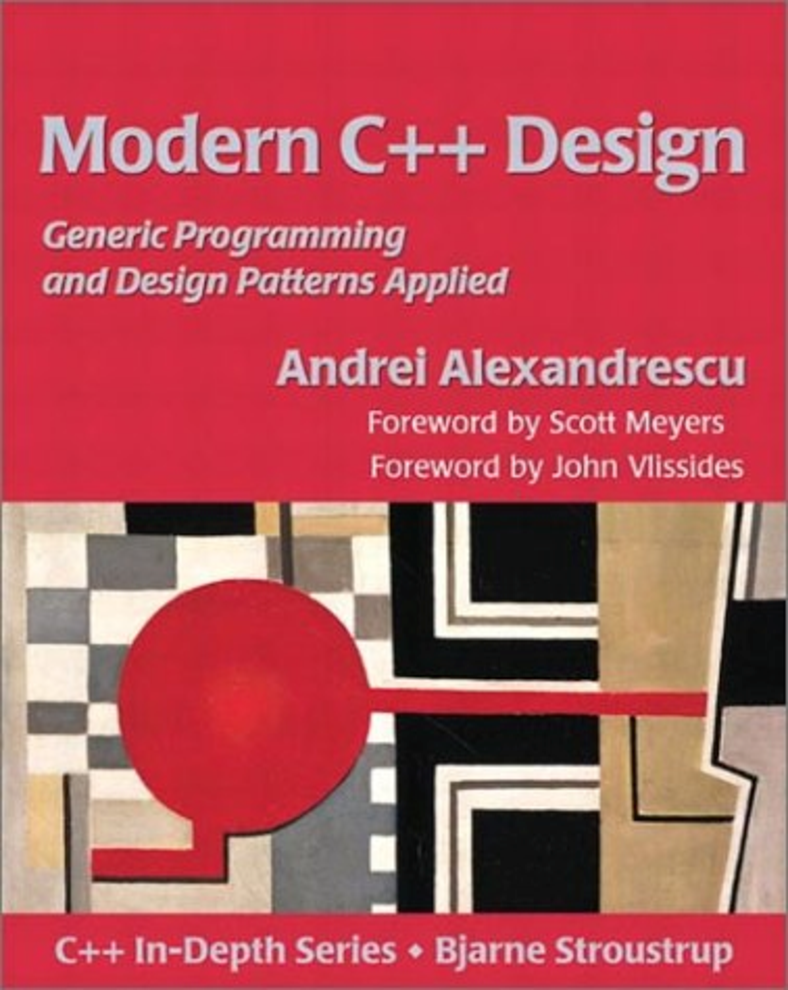
\includegraphics[width=4.5cm]{modern-cxx.pdf}
    \end{column}
    \begin{column}{.5\textwidth}
      \centering 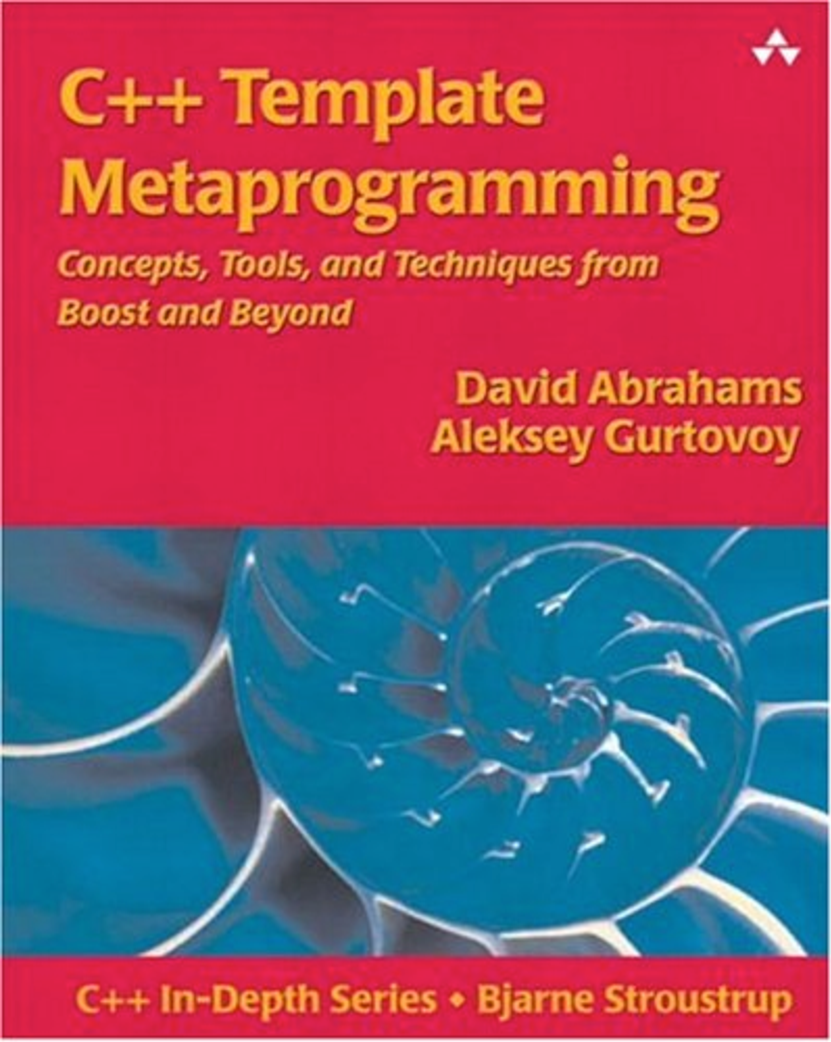
\includegraphics[width=4.5cm]{cxx-template.pdf}
    \end{column}
  \end{columns}
\end{frame}

\subsection*{\redm\whitem\greenb}
\begin{frame}
  \frametitle{ALPSの展開}
  \begin{itemize}
    \setlength{\itemsep}{1em}
  \item 上方展開 (大規模化・高性能化・並列化)
    \begin{itemize}
    \item 量子モンテカルロ法(ALPS/looper)の超並列化
    \item 高並列スケジューラ(ALPS/parapack)のハイブリッド多重並列化
    \item Fortran, C プログラムのための API 作成
    \end{itemize}
  \item 下方展開 (裾野を広げる)
    \begin{itemize}
    \item 実験家・理論家による幅広い利用の促進
    \item Windows/Macintosh 用バイナリインストーラの開発
    \item ワークフロー・履歴管理システムとの統合
    \item GUI (グラフィカルユーザインターフェース)の開発
    \end{itemize}
  \end{itemize}
\end{frame}

\subsection*{\redm\whitem\greenb}
\begin{frame}
  \frametitle{開発のためのインフラストラクチャ}
  \begin{itemize}
  \item ソースコードの規模, 開発体制が大きくなると今までの方法では破綻する
  \item 開発・サポートのためのツールを一から作りあげるのは非現実的
  \item フリーソフトウェアの利用
    \begin{itemize}
    \item ビルドシステム: CMake
    \item ソースコードの管理: Subversion
    \item プロジェクト管理・バグ追跡: Trac
    \item ドキュメント作成: MediaWiki
    \item メーリングリスト: Mailman
    \end{itemize}
  \item Linux ワークステーションが1台あれば, これらの環境を整えるのは現在では比較的容易
  \end{itemize}
\end{frame}

\subsection*{\redm\whitem\greenb}
\begin{frame}
  \frametitle{ビルドシステム: CMake}
  \begin{itemize}
    \setlength{\itemsep}{1em}
  \item Makefileを生成するためのユーティリティー (configureスクリプトに対応)
    \begin{itemize}
    \item Windows の Visual C++ 用ソリューションファイル, Mac OS X の Xcode 用プロジェクトファイルの生成も可能
    \end{itemize}
  \item 設定は CMakeLists.txt に記述する
  \item テスト(CTest)やバイナリ配布(CPack)の機能もある
  \item ファイルの依存関係の自動検出
  \end{itemize}
\end{frame}

\subsection*{\redm\whitem\greenb}
\begin{frame}
  \frametitle{VCS (Version Control System)によるソース管理: Subversion}
  \begin{itemize}
  \item 開発者が複数になると, ディレクトリ名やログファイルによるバージョン管理はすぐに破綻する
  \item ソースコードをサーバー上で一括管理
    \begin{itemize}
    \item ネットワーク経由でソースを check out/check in
    \end{itemize}
  \item 更新毎に一意なバージョン番号を付与
  \item 全ての修正履歴を保存
  \item 複数人が同時に更新した場合に衝突を回避するしくみ
  \item ブランチ・マージ・タグ付けなどが可能
  \item 開発者が一人, 公開の予定がない場合でも積極的に使うべき
  \end{itemize}
\end{frame}

\subsection*{\redm\whitem\greenb}
\begin{frame}
  \frametitle{BTS (Bug Tracking System) の利用: Trac}
  \begin{itemize}
    \setlength{\itemsep}{1em}
  \item プロジェクト管理とバグ追跡のためのツール
  \item Web ブラウザからアクセス・操作
    \begin{itemize}
    \item 開発者の情報共有のための wiki
    \item Subversion との連携 (ソース, 修正履歴の web 上での閲覧)
    \item プロジェクト管理 (ロードマップ, マイルストーンの管理)
    \item チケットシステム: バグやタスクの登録, 担当者の決定, 修正状況の追跡
    \end{itemize}
  \end{itemize}
\end{frame}

\subsection*{\redm\whitem\greenb}
\begin{frame}
  \frametitle{Wikiによるマニュアル作成: MediaWiki}
  \begin{itemize}
  \item もともとはウィキペディアのために開発された
  \item Wiki とは?
    \begin{itemize}
    \item Webブラウザを利用してWeb文書を書き換えるシステム
    \item ネットワーク上のどこからでも書き換えができる
    \item 共同作業が容易
    \item Webブラウザがあれば編集作業が行える
    \item HTMLよりも簡潔な書式
    \item 文書間のリンクの作成が容易
    \end{itemize}
  \item ALPS Wiki のコンテンツ
    \begin{itemize}
    \item ニュース, インストール方法, ALPSに関連する論文, 発表資料, ライブラリリファレンスマニュアル, チュートリアル
    \end{itemize}
  \end{itemize}
\end{frame}

\subsection*{\redm\whitem\greenb}
\begin{frame}
  \frametitle{メーリングリストの活用: Mailman}
  \begin{itemize}
    \setlength{\itemsep}{1em}
  \item 開発者メーリングリスト
    \begin{itemize}
    \item 開発方針に関する意見交換, リリーススケジュール調整, 担当者調整等
    \item Trac チケットの変更ログも自動的にここに流れる
    \end{itemize}
  \item ユーザメーリングリスト
    \begin{itemize}
    \item Web からの自動登録
    \item 開発者 + ユーザコミュニティーによるサポートの場
    \item FAQ ⇒ Wiki ドキュメントへ反映
    \item バグレポート, 要望など ⇒ Trac チケットへ
    \end{itemize}
  \end{itemize}
\end{frame}

\section{ALPSize (ALPS化)のすすめ}

\subsection*{\redm\whitem\greenb}
\begin{frame}
  \frametitle{ALPSライブラリを使用する利点}
  \begin{itemize}
  \item エラーバーと自己相関時間の自動計算 (ALPS/alea)
  \item 自動並列化 \& ロードバランシング (ALPS/scheduler)
  \item チェックポイント作成とリスタート機能 (ALPS/scheduler)
  \item XML形式による計算結果の自動出力とこれらを扱うコマンドラインツール
  \item 入力パラメータの柔軟な扱い (ALPS/parameter)
  \item 擬似乱数生成器 (ALPS/random)
  \item 格子の容易な取扱い (ALPS/lattice)
  \item 量子ハミルトニアンの容易な取扱い (ALPS/model)
  \end{itemize}
\end{frame}

\subsection*{\redm\whitem\greenb}
\begin{frame}
  \frametitle{ALPSビルド環境を使用する利点}
  \begin{itemize}
  \item コンパイラ \& 最適化オプションの自動設定
  \item MPI \& OpenMP用オプションの自動設定
  \item ライブラリ(Boost, BLAS/LAPACK, HDF5, FFTW, SQLite, Python等)の自動検出
  \item ALPSライブラリを利用するためのオプションの自動設定
  \item テスト用スクリプト
  \item 京、FX10、その他代表的なスパコン用のビルド環境が整備されている
  \item Windows用のバイナリ作成が可能
  \end{itemize}
\end{frame}

\subsection*{\redm\whitem\greenb}
\begin{frame}
  \frametitle{ALPSize実習}
  \begin{itemize}
    \setlength{\itemsep}{1em}
  \item 00-01 ALPSビルド環境の利用 (Make, CMake)
  \item 02-05 C++プログラミング
  \item 06-08 ALPSライブラリの利用
  \item 09 ALPSスケジューラの利用
  \end{itemize}
\end{frame}

\section{ALPSビルド環境}

\subsection*{\redm\whitem\greenb}
\begin{frame}[c,fragile]
  \frametitle{ビルド環境のセットアップ}
  \begin{itemize}
    \setlength{\itemsep}{1em}
  \item 環境変数の設定
    \begin{itemize}
    \item {\color{red} ALPS\_HOME}: ALPSがインストールされているディレクトリ\\ (例: /usr/local/alps)
    \item {\color{red} PATH}: ツール(parameter2xml)のパスを追加
    \item {\color{red} LD\_LIBRARY\_PATH}: ALPSライブラリのパスを設定
    \item {\color{red} PYTHONPATH}: ALPS Pythonモジュールのパスを追加
    \end{itemize}
  \item ALPSがプレインストールされている環境では、上記の設定を行うシェルスクリプトが用意されている. 例)
\begin{lstlisting}
$ source /usr/local/alps/bin/alpsvars.sh
\end{lstlisting}
  \end{itemize}
\end{frame}

\subsection*{\redm\whitem\greenb}
\begin{frame}[c,fragile]
  \frametitle{Makeの利用}
  \begin{itemize}
  \item \$ALPS\_HOME/share/alps/include.mk に Makefile 用の変数設定ファイルが用意されている
  \item Makefileの例
\begin{lstlisting}
include $(ALPS_HOME)/share/alps/include.mk
hello: hello.C
        $(CXX) $(CPPFLAGS) $(CXXFLAGS) $(LDFLAGS) -o hello hello.C $(LIBS)
\end{lstlisting}
  \item 実習
\begin{lstlisting}
$ cp -r $ALPS_HOME/tutorials/alpsize-00-make $HOME
$ cd $HOME/alpsize-00-make
$ make
\end{lstlisting}
  \item {\color{blue} CMake の利用を推奨}
  \end{itemize}
\end{frame}

\subsection*{\redm\whitem\greenb}
\begin{frame}
  \frametitle{CMake}
  \begin{itemize}
    \setlength{\itemsep}{1em}
  \item クロスプラットフォームなビルドツール \\
    Windowsにも対応
  \item Makefileを生成
  \item 高速な並列ビルド
  \item テスト環境
  \item ビルドルール, ライブラリ, 依存関係などは CMakeLists.txt に記述する
  \end{itemize}
\end{frame}

\subsection*{\redm\whitem\greenb}
\begin{frame}[c,fragile]
  \frametitle{01 CMake化}
  \begin{itemize}
    \setlength{\itemsep}{1em}
  \item 簡単なプログラムをCMakeを利用してビルドする
\begin{lstlisting}
$ mkdir $HOME/alpsize-01-cmake
$ cd $HOME/alpsize-01-cmake
$ cmake $ALPS_HOME/tutorials/alpsize-01-cmake
$ make
$ ctest
$ ./hello
\end{lstlisting}
  \item {\color{red} CMakeではソースディレクトリ(\$ALPS\_HOME/tutorials/alpsize-01-cmake)とビルドディレクトリ(\$HOME/alpsize-01-cmake)は別にする}
  \end{itemize}
\end{frame}

\subsection*{\redm\whitem\greenb}
\begin{frame}[fragile,shrink=20]
  \frametitle{CMakeLists.txtの例}
  {\small \$ALPS\_HOME/tutorials/alpsize-01-cmake/CMakeLists.txt}
\begin{semiverbatim}
\alert<1>{cmake_minimum_required(VERSION 2.8 FATAL_ERROR)}
\alert<1>{project(hello NONE)}

# find ALPS Library
\alert<1>{find_package(ALPS REQUIRED PATHS $\{ALPS_ROOT_DIR\} $ENV\{ALPS_HOME\}
          NO_SYSTEM_ENVIRONMENT_PATH)}
\alert<1>{message(STATUS "Found ALPS: $\{ALPS_ROOT_DIR\} (revision: $\{ALPS_VERSION\})")}
\alert<1>{include($\{ALPS_USE_FILE\})}

# enable C and C++ compilers
\alert<2>{enable_language(C CXX)}

# rule for generating 'hello world' program
\alert<3>{add_executable(hello hello.C)}
\alert<3>{target_link_libraries(hello $\{ALPS_LIBRARIES\})}
\alert<4>{add_alps_test(hello)}
\end{semiverbatim}
\end{frame}

\subsection*{\redm\whitem\greenb}
\begin{frame}[fragile,shrink]
  \frametitle{テストスクリプト}
add\_alps\_testは以下と同等
\begin{semiverbatim}
$ ./hello \$ALPS_HOME/tutorials/alpsize-00-CMake/hello.ip \\
  > hello.tmp
$ diff -u \$ALPS_HOME/tutorials/alpsize-00-CMake/hello.op \\
  hello.tmp
$ rm hello.tmp
\end{semiverbatim}
実行結果(出力)を hello.op と比較
\begin{semiverbatim}
\$ cat \$ALPS_HOME/tutorials/alpsize-00-CMake/hello.op
hello, world
\end{semiverbatim}
\end{frame}

\section{C++プログラミング}

\subsection*{\redm\whitem\greenb}
\begin{frame}[fragile]
  \frametitle{02 Cプログラム}
  \begin{itemize}
    \item Wolffアルゴリズム
      \begin{itemize}
        \item 2次元正方格子強磁性Ising模型のモンテカルロ計算
        \item ランダムに選んだ点からクラスターを作成し, スピン反転
        \item ソースコード: \href{https://github.com/cmsi/alps-tutorial/blob/develop/alpsize/02-wolff.c}{wolff.c}
      \end{itemize}
    \item ビルドと実行
\begin{lstlisting}
$ mkdir $HOME/alpsize-02-original-c
$ cd $HOME/alpsize-02-original-c
$ cmake $ALPS_HOME/tutorials/alpsize-02-original-c
$ make
$ ./wolff
\end{lstlisting}
\end{itemize}
\end{frame}

\subsection*{\redm\whitem\greenb}
\begin{frame}[fragile]
  \frametitle{03 C++プログラム}
  \begin{itemize}
    \item WolffアルゴリズムC++で書きなおす
      \begin{itemize}
        \item ヘッダファイル名, namespace, コメント形式
        \item for 文中でのループ変数の宣言
        \item iostream を用いた結果の出力
        \item 修正点: \href{https://github.com/cmsi/alps-tutorial/blob/develop/alpsize/03-wolff.diff}{wolff.diff}
      \end{itemize}
    \item ビルドと実行
\begin{lstlisting}
$ mkdir $HOME/alpsize-03-basic-cpp
$ cd $HOME/alpsize-03-basic-cpp
$ cmake $ALPS_HOME/tutorials/alpsize-03-basic-cpp
$ make
$ ./wolff
\end{lstlisting}
  \end{itemize}
\end{frame}

\subsection*{\redm\whitem\greenb}
\begin{frame}[fragile]
  \frametitle{04 STLの利用}
  \begin{itemize}
    \item STL (C++ Standard Template Library)を利用する
      \begin{itemize}
        \item std::vector : 動的配列
        \item std::stack : pop, push, top, empty メンバ関数
        \item 修正点: \href{https://github.com/cmsi/alps-tutorial/blob/develop/alpsize/04-wolff.diff}{wolff.diff}
      \end{itemize}
    \item ビルドと実行
\begin{lstlisting}
$ mkdir $HOME/alpsize-04-stl
$ cd $HOME/alpsize-04-stl
$ cmake $ALPS_HOME/tutorials/alpsize-04-stl
$ make
$ ./wolff
\end{lstlisting}
  \end{itemize}
\end{frame}

\subsection*{\redm\whitem\greenb}
\begin{frame}[fragile]
  \frametitle{05 Boostの利用}
  \begin{itemize}
    \item Boostライブラリを利用する
      \begin{itemize}
        \item \href{http://boost.org/doc/html/array.html}{boost::array} : 固定長配列
        \item \href{http://boost.org/doc/html/boost_random.html}{boost::random} : 擬似乱数生成器, 確率分布
        \item boost::timer : ポータブルなタイマー
        \item 修正点: \href{https://github.com/cmsi/alps-tutorial/blob/develop/alpsize/05-wolff.diff}{wolff.diff}
      \end{itemize}
    \item ビルドとテスト
\begin{lstlisting}
$ mkdir $HOME/alpsize-05-boost
$ cd $HOME/alpsize-05-boost
$ cmake $ALPS_HOME/tutorials/alpsize-05-boost
$ make
$ ctest
\end{lstlisting}
  \end{itemize}
\end{frame}

%% \begin{frame}[fragile,shrink=10]
%%   \frametitle{04 Boostの利用 (2)}
%% \begin{semiverbatim}
%% ...
%% #include <boost/random.hpp>
%% ...
%% // random number generator
%% boost::mt19937 eng(SEED);
%% boost::variate_generator<boost::mt19937&, boost::uniform_real<> >
%% random_01(eng, boost::uniform_real<>());
%% \end{semiverbatim}
%% \end{frame}

\section{ALPSライブラリの利用}

\subsection*{\redm\whitem\greenb}
\begin{frame}[fragile]
  \frametitle{06 ALPS/parameters}
  \begin{itemize}
    \item ALPS/parameterライブラリを利用する
      \begin{itemize}
        \item 標準入力から, 変数名と値のペアを読み込む. 値は「式」でも良い
        \item alps::Parameter, alps::Parameters, alps::ParameterList
        \item デフォルト値の設定
        \item 修正点: \href{https://github.com/cmsi/alps-tutorial/blob/develop/alpsize/06-wolff.diff}{wolff.diff}
      \end{itemize}
    \item ビルドとテスト
\begin{lstlisting}
$ mkdir $HOME/alpsize-06-parameters
$ cd $HOME/alpsize-06-parameters
$ cmake $ALPS_HOME/tutorials/alpsize-06-parameters
$ make
$ ctest
\end{lstlisting}
  \end{itemize}
\end{frame}

\subsection*{\redm\whitem\greenb}
\begin{frame}[fragile]
  \frametitle{ALPS/parameterライブラリ}
  プログラムに与えるパラメータを解釈するライブラリ
  \begin{columns}
    \begin{column}{6cm}
\begin{semiverbatim}
LATTICE = "chain lattice";
L = 16,

SEED = 2873
// C++ style comment
SWEEPS = 4096;
THERMALIZATION = \alert<1>{SWEEPS/8};
/* C style comment */
\{ T = 2; Sq = 2*\alert<2>{PI}/3; \}
\{ T = 1.8; \}
\end{semiverbatim}
    \end{column}
    \begin{column}{6cm}
      \begin{itemize}
      \item 四則演算可能
      \item $\pi$ を文字で指定
      \item 空行も正しく認識
      \item C風, C++風のコメント
      \item \{ \} で囲んだ変数は異なるセット
      \item 空白を適切に認識
      \item 改行, セミコロン, コンマで変数を区別
      \end{itemize}
    \end{column}
  \end{columns}
\end{frame}

\subsection*{\redm\whitem\greenb}
\begin{frame}[fragile,shrink=5]
\frametitle{ALPS/parameterライブラリの利用法}
\begin{semiverbatim}
#include <boost/foreach.hpp>
#include <alps/parameter.h>
...
int main(int argc, char** argv) \{
...
  alps::ParameterList plist = read_param(argc, argv);
  BOOST_FOREACH(alps::Parameters& p, plist) \{
    \alert<1>{double a = p["a"];}
    \alert<2>{double b = p.value_or_default("b", 0.5);}
...
  \}
...
\}
\end{semiverbatim}
\end{frame}

\subsection*{\redm\whitem\greenb}
\begin{frame}[fragile]
  \frametitle{07 ALPS/alea}
  \begin{itemize}
    \item ALPS/aleaライブラリを利用する
      \begin{itemize}
        \item マルコフ連鎖における平均値, エラーバー, 自己相関を計算するライブラリ
        \item 非線形な量についても, ジャックナイフ法を用いて正しいエラーバーを評価可能 (例: Binder比 $\langle m^2 \rangle^2 / \langle m^4 \rangle$)
        \item 修正点: \href{https://github.com/cmsi/alps-tutorial/blob/develop/alpsize/07-wolff.diff}{wolff.diff}
      \end{itemize}
    \item ビルドとテスト
\begin{lstlisting}
$ mkdir $HOME/alpsize-07-alea
$ cd $HOME/alpsize-07-alea
$ cmake $ALPS_HOME/tutorials/alpsize-07-alea
$ make
$ ctest
\end{lstlisting}
  \end{itemize}
\end{frame}

\subsection*{\redm\whitem\greenb}
\begin{frame}[fragile,shrink=10]
  \frametitle{ALPS/aleaライブラリの利用法}
  マルコフ連鎖における平均値, 分散, 自己相関を計算するライブラリ
\begin{semiverbatim}
#include <alps/alea.h>
...
alps::ObservableSet obs;
...
obs << alps::RealObservable("Energy");
...
for (int i = 0; i != N; ++i) \{
  double e = energy(); // calclulate something
  obs.reset(i == THERM); // when thermalized
  obs["Energy"] << e;
\}
...
std::cout << obs["Energy"];
\end{semiverbatim}
\end{frame}

\subsection*{\redm\whitem\greenb}
\begin{frame}[fragile,shrink=10]
\frametitle{Tips: 出力を制御する}
\begin{semiverbatim}
// Gnuplot 風出力
std::cout << 1./param["beta"] << " "
          << obs["Energy"].mean() << " "
          << obs["Energy"].variance() << std::endl;
\end{semiverbatim}
\end{frame}

\subsection*{\redm\whitem\greenb}
\begin{frame}[fragile]
  \frametitle{08 ALPS/lattice}
  \begin{itemize}
    \item ALPS/latticeライブラリを利用する
      \begin{itemize}
        \item XMLにより任意の次元の任意の格子(グラフ)を生成可
        \item サイト数, ボンド数, 全サイト, 全ボンド, 最近接サイト, etc へのアクセス関数
        \item 修正点: \href{https://github.com/cmsi/alps-tutorial/blob/develop/alpsize/08-wolff.diff}{wolff.diff}
      \end{itemize}
    \item ビルドとテスト
\begin{lstlisting}
$ mkdir $HOME/alpsize-08-lattice
$ cd $HOME/alpsize-08-lattice
$ cmake $ALPS_HOME/tutorials/alpsize-08-lattice
$ make
$ ctest
\end{lstlisting}
  \end{itemize}
\end{frame}

\subsection*{\redm\whitem\greenb}
\begin{frame}[fragile] \frametitle{ALPS/latticeライブラリの利用法}
\begin{semiverbatim}
#include <alps/lattice.h>
...
class ising : public alps::graph_helper<> \{
 public:
  ising(alps::Parameters const& p)
   : \alert{graph_helper<>(p)} \{\}
...
\};
\end{semiverbatim}
\end{frame}

\subsection*{\redm\whitem\greenb}
\begin{frame}[fragile,shrink=30]
  \frametitle{格子(graph)の定義}
\begin{semiverbatim}
<LATTICE name="square lattice" dimension="2">
  <PARAMETER name="a" default="1"/>
  <BASIS><VECTOR>a 0</VECTOR><VECTOR>0 a</VECTOR></BASIS>
  <RECIPROCALBASIS><VECTOR>2*pi/a 0</VECTOR><VECTOR>0 2*pi/a</VECTOR></RECIPROCALBASIS>
</LATTICE>
<UNITCELL name="simple2d" dimension="2">
  <VERTEX/>
  <EDGE><SOURCE vertex="1" offset="0 0"/><TARGET vertex="1" offset="0 1"/></EDGE>
  <EDGE><SOURCE vertex="1" offset="0 0"/><TARGET vertex="1" offset="1 0"/></EDGE>
</UNITCELL>
<LATTICEGRAPH name = "square lattice">
  <FINITELATTICE>
    <LATTICE ref="square lattice"/>
    <PARAMETER name="W" default="L"/>
    <EXTENT dimension="1" size="L"/>
    <EXTENT dimension="2" size="W"/>
    <BOUNDARY type="periodic"/>
  </FINITELATTICE>
  <UNITCELL ref="simple2d"/>
</LATTICEGRAPH>
\end{semiverbatim}
\end{frame}

\subsection*{\redm\whitem\greenb}
\begin{frame}[fragile,shrink=10]
  \frametitle{ALPS/latticeライブラリの便利な関数}
\begin{semiverbatim}
std::vector<double> d(\alert{num_sites()});
std::vector<double> J(\alert{num_bonds()});
...
double energy = 0.;
BOOST\_FOREACH(site_descriptor s, \alert{sites()}) \{
  BOOST\_FOREACH(bond_descriptor b, \alert{neighbor_bonds(s)}) \{
    energy += J[b] * d[\alert{source(b)}] * d[\alert{target(b)}];
  \}
\}
...
boost::mt19937 rng;
boost::uniform_int<> dst(0, \alert{num_bonds()}-1);
J[\alert{bond(dst(rng))}] = 0;
Jtemp = param["J" + \alert{bond_type(b)}];
\end{semiverbatim}
  \begin{itemize}
  \item sites(), bonds() は BOOST\_FOREACH と組み合わせる
  \item index(s) や index(b) で数字に変換
  \item bond(n) や site(n) で *\_descriptor に変換
  \end{itemize}
\end{frame}

\section{ALPSスケジューラの利用}

\subsection*{\redm\whitem\greenb}
\begin{frame}[fragile]
  \frametitle{09 ALPS Scheduler (1)}
  \begin{itemize}
    \item ALPSには3種類のスケジューラ. 本講習ではALPS/parapackスケジューラを使用
    \item ユーザのシミュレーションコードをWorkerクラスにカプセル化 (例: \href{https://github.com/cmsi/alps-tutorial/blob/develop/alpsize/09-hello_worker.h}{hello\_worker.h})
    \item Workerクラスが実装しなければならない関数
      \begin{itemize}
        \item コンストラクタ、init\_obserbablesメンバー関数
        \item runメンバー関数
        \item is\_thermalized \& progressメンバ関数
        \item save \& loadメンバ関数
      \end{itemize}
    \item PARAPACK\_REGISTER\_WORKERマクロを用いてWorkerをスケジューラに登録 (例: \href{https://github.com/cmsi/alps-tutorial/blob/develop/alpsize/09-hello_worker.C}{hello\_worker.C})
    \item 実行時にALGORITHMパラメータでWorkerを選択できる
  \end{itemize}
\end{frame}

\subsection*{\redm\whitem\greenb}
\begin{frame}[fragile]
  \frametitle{09 ALPS Scheduler (2)}
  \begin{itemize}
    \item メイン文: \href{https://github.com/cmsi/alps-tutorial/blob/develop/alpsize/09-wolff.C}{worker.C})
\begin{lstlisting}
int main(int argc, char** argv) {
  return alps::parapack::start(argc, argv);
}
\end{lstlisting}
    \item ビルド, テスト, (マルチスレッド)実行
\begin{lstlisting}
$ mkdir $HOME/alpsize-09-scheduler
$ cd $HOME/alpsize-09-scheduler
$ cmake $ALPS_HOME/tutorials/alpsize-09-scheduler
$ make
$ ctest
$ parameter2xml $ALPS_HOME/.../wolff_params wolff_params
$ ./wolff wolff_params.in.xml
\end{lstlisting}
  \end{itemize}
\end{frame}

\subsection*{\redm\whitem\greenb}
\begin{frame}[fragile]
  \frametitle{09 ALPS Scheduler (3)}
  \begin{itemize}
    \item Workerの一生
      \begin{itemize}
        \item 初回: コンストラクタ $\Rightarrow$ {\color{red} init\_observables} $\Rightarrow$ run $\Rightarrow$ run $\Rightarrow$ run  $\Rightarrow$ $\cdots$ $\Rightarrow$ save $\Rightarrow$ デストラクタ
        \item チェックポイントリスタート後: コンストラクタ $\Rightarrow$ {\color{red} load} $\Rightarrow$ run $\Rightarrow$ run $\Rightarrow$ run  $\Rightarrow$ $\cdots$ $\Rightarrow$ save  $\Rightarrow$ デストラクタ
      \end{itemize}
      \item init\_observablesは初回のみ呼び出される
      \item progressの返り値が1に達する or 制限時間に達するまで run が繰り返し呼ばれる
      \item 定期的にsave関数が呼ばれる
  \end{itemize}
\end{frame}

\subsection*{\redm\whitem\greenb}
\begin{frame}[fragile]
  \frametitle{09 ALPS Scheduler (4)}
  \begin{itemize}
    \item コンストラクタ: worker(alps::Parameters const\&);
      \begin{itemize}
        \item パラメタの読み込み、配列の初期化など
      \end{itemize}
    \item init\_observables(alps::Parameters const\&, alps::ObservableSet\& obs);
      \begin{itemize}
        \item 物理量の宣言 \& 登録
      \end{itemize}
    \item run(alps::ObservableSet\&);
      \begin{itemize}
        \item 何らかの計算を1ステップだけ実行
      \end{itemize}
    \item bool is\_thermalized() const;
      \begin{itemize}
        \item この値がtrueの間だけ物理量が保存される. (falseからtrueに変わった時点でリセットされる)
      \end{itemize}
    \item double progress() const;
      \begin{itemize}
        \item 進捗状況を [0,1] で返す
      \end{itemize}
  \end{itemize}
\end{frame}

\subsection*{\redm\whitem\greenb}
\begin{frame}[fragile]
  \frametitle{09 ALPS Scheduler (5)}
  \begin{itemize}
    \item save(alps::ODump\&) const;
      \begin{itemize}
        \item チェックポイントの書き出し. スピン配位などをバイナリ形式(xdr)で保存する
        \item alps::ODump には, int, double, std::vector 等ほとんど何でも書き込める
        \item ユーザが宣言した構造体, クラスのインスタンスを書き込みたい場合には, 演算子をオーバーロードする
\begin{lstlisting}
dp << mcs << spin << sz;
\end{lstlisting}
      \end{itemize}
    \item load(alps::IDump\&);
      \begin{itemize}
        \item チェックポイントからの読み込み
        \item 書き出しと同じ順序で読み込む
\begin{lstlisting}
dp >> mcs >> spin >> sz;
\end{lstlisting}
      \end{itemize}
  \end{itemize}
\end{frame}

\subsection*{\redm\whitem\greenb}
\begin{frame}[fragile]
  \frametitle{09 ALPS Scheduler (6)}
  \begin{itemize}
    \item Workerの基底クラス
      \begin{itemize}
      \item alps::parapack::abstract\_worker : 最も基本的な基底クラス
      \item alps::parapack::mc\_worker : alps::rng\_helper を継承. 乱数生成器が利用可. 乱数生成器の状態のチェックポイントリスタートも自動的に行われる
      \item alps::parapack::lattice\_mc\_worker$\langle\rangle$ : alps::graph\_helper を継承. ALPS/latticeライブラリの関数が利用可
      \item alps::parapack::latticemodel\_mc\_worker$\langle\rangle$ : alps::protected model\_helper$\langle\rangle$ を継承. ALPS/modelライブラリの関数が利用可
      \end{itemize}
  \end{itemize}
\end{frame}

\subsection*{\redm\whitem\greenb}
\begin{frame}[fragile]
  \frametitle{09 ALPS Scheduler (7)}
  \begin{itemize}
    \item Evaluator: \href{https://github.com/cmsi/alps-tutorial/blob/develop/alpsize/09-wolff_worker.h}{wolff\_worker.h}
      \begin{itemize}
      \item ALPS/parapackスケジューラでは, NUM\_CLONESパラメータを指定することで, 同じパラメータセットで乱数の種だけが異なるシミュレーション(Clone)を複数並列実行可 (ばかパラ)
      \item 同じパラメータセットに属するCloneの測定量は, 終了時に自動的にマージされる
      \item 非線形な物理量(例: ビンダー比, 相関長)の計算は、Cloneのマージが終わった後に行う必要がある
      \item EvaluatorをWorkerと同じ名前でスケジューラに登録しておくと, Cloneのマージ後にevaluate関数が呼び出される
      \end{itemize}
  \end{itemize}
\end{frame}

\subsection*{\redm\whitem\greenb}
\begin{frame}[fragile]
  \frametitle{09 ALPS Scheduler (8)}
  \begin{itemize}
    \item Workerの並列化 (OpenMP並列)
      \begin{itemize}
      \item CMake時に, -DALPS\_ENABLE\_OPENMP\_WORKER=ON が指定されていれば、Workerの中でOpenMP利用可
      \end{itemize}
    \item Workerの並列化 (MPI並列)
      \begin{itemize}
      \item Workerのコンストラクタを修正
\begin{lstlisting}
worker(mpi::communicator const&, alps::Parameters const&)
\end{lstlisting}
      \item コンストラクタに渡された mpi::communicator の中は自由に使ってよい.
      \item {\color{red} PARAPACK\_REGISTER\_PARALLEL\_WORKER}マクロを用いてWorkerを登録
      \end{itemize}
    \item 実行時に -r オプションと -p オプションで, 総スレッド数とWorkerあたりのスレッド数を指定
  \end{itemize}
\end{frame}

\subsection*{\redm\whitem\greenb}
\begin{frame}[fragile]
  \frametitle{10,11 ALPS Fortran}
  \begin{itemize}
  \item FortranプログラムをALPSに組み込む
    \begin{itemize}
      \item クラスの代わりにサブルーチン群を作成する (alps\_init, alps\_init\_observable, alps\_run, など)
      \item サブルーチン間の状態の受け渡しは, common または module を利用する
      \item C++ポインタの受け渡しに integer(2) を使う (caller変数)
    \end{itemize}
  \item チュートリアル
  \begin{itemize}
    \item \href{http://alps.comp-phys.org/mediawiki/index.php/Tutorials:ALPS_Fortran_Introduction/ja}{ALPS Fortran Introduction}
    \item \href{http://alps.comp-phys.org/mediawiki/index.php/Tutorials:ALPS_Fortran_Application_Development/ja}{ALPS Fortran Application Development}
  \end{itemize}
  \end{itemize}
\end{frame}

\subsection*{\redm\whitem\greenb}
\begin{frame}[fragile]
  \frametitle{実習}
  \begin{itemize}
    \setlength{\itemsep}{1em}
  \item 逐次プログラムのALPS化
    \begin{itemize}
      \item オリジナルコード: \href{https://github.com/cmsi/alps-tutorial/blob/develop/alpsize/ising.C}{ising.C}
    \end{itemize}
  \item 並列プログラムのALPS化
    \begin{itemize}
      \item オリジナルコード: \href{https://github.com/cmsi/alps-tutorial/blob/develop/alpsize/ising_parallel.C}{ising\_parallel.C}
    \end{itemize}
  \end{itemize}
\end{frame}

\end{document}
